\section{TP7 Apply the Web instead of working around}
\label{sec:principle-tp7-apply-the-web}

Der moderne Internetbrowser kapselt eine Vielzahl von leistungsfähigen Funktionen des jeweiligen Hostrechners in ein für den Software Entwickler leicht zu verwendendes Interface. Die Integration von systemnahen Komponenten wie \gls{GPU}'s \cite{webgl} gehört dabei genauso dazu wie die Möglichkeit, gleichzeitig mehrere Fenster oder Tabs für dieselbe oder auch verschiedene Applikationen resp. Internetseiten offen zu halten.

Das Hin- und Herspringen zwischen besuchten Seiten mittels Vorwärts- und Zurück-Schaltflächen gehört seit Beginn der Web-Ära zum festen Bestandteil der User Experience im Internet.

In der Vergangenheit gehörten wiederkehrende Umsetzungen von Funktionen wie der Validierung von Formularinhalten zu lästigen, aber nötigen Ärgernissen. Mit der Einführung der neusten Revision 5 des HTML Standards können gerade solche Aufgaben bequem dem Browser \cite{HTML5Forms} überlassen werden

Mit der immer mächtiger werdenden Formatierungssprache CSS und dessen neuster Version 3 sind heute gestalterische Effekte möglich, welche bis vor Kurzem nur mittels umständlicher Einbindung von Grafikdateien (Stichwort Schlagschatten \cite{css-box-shadow} oder Farbverläufen \cite{css-gradient}) möglich waren.

Mit der Richtlinie \emph{TP7} hält Stefan Tilkov Software Entwickler dazu an, die Werkzeuge welche vom Internetbrowser angeboten werden, gewinnbringend zu nutzen.


\subsection*{Geplante Umsetzung}

In der Beispielapplikation sollen gezielt HTML 5 Features verwendet werden:

\begin{itemize}
	\item Semantisch korrekte Tags (\emph{<header>}, \emph{<section>} etc., siehe auch \ref{sec:principle-rp11-posh} ``\nameref{sec:principle-rp11-posh}'')
	\item Formularvalidierung \cite{HTML5Forms}
\end{itemize}

Das entstehende, semantisch korrekte HTML Markup soll mit CSS 3 gestaltet werden. Neue Möglichkeiten zur grafischen Darstellung sollen ausgenutzt werden. Die Verwendung von \emph{Responsive Design} resp. den zugrundeliegenden \emph{Media Queries} \cite{css-mediaquery} soll die  Darstellung auf verschiedenen Bildschirmen (Desktops, Tablets, Smartphones usw.) optimieren und vereinfachen.

Bei der Entwicklung der Front- als auch Backend-Komponente muss, wie von \ref{sec:principle-rp18-history-api} ``\nameref{sec:principle-rp18-history-api}'' bereits gefordert, zwingend darauf geachtet werden, dass die Verwendung der Browser-Funktionen \emph{Vorwärts}, \emph{Zurück} und \emph{Aktualisieren} zu keinem unerwarteten Verhalten führt.

\subsection*{Konkrete Umsetzung}

\subsubsection*{HTML Markup}

Wie geplant verwendet das gerenderte HTML Markup die vom HTML 5 Standard eingeführten Funktionen. Quelltext \ref{lst:roomiesMenuHtml} zeigt die Verwendung des \emph{<header>} sowie \emph{<nav>} Tags zur Beschreibung des Applikationsmenüs der Beispielapplikation.

\begin{lstlisting}[language=HTML, caption={Ausschnitt des gerenderten HTML Markups der Menüleiste \emph{Roomies}}, label={lst:roomiesMenuHtml}]
<header id="menu">
	<div class="fixed-navigation">
		<nav class="navigation" role="navigation">
			<div class="title-area">
				<a href="/" class="banner" title="Roomies"><h1>Roomies</h1></a>
			</div>
			<section class="nav-section">
				<ul class="left">
						<li>
							<a href="/community/ba-team/tasks" title="Aufgaben">
								<i class="icon-tasks icon-large"></i>
								<span class="item-label"> Aufgaben</span>
							</a>
						</li>
						<!-- ... more items -->
				</ul>
				<!-- ... displaying the facebook profile picture -->
			</section>
		</nav>
	</div>
</header>
\end{lstlisting}

Weiter wurde für das \emph{Fällig bis}-Feld auf der Ansicht \emph{Aufgabe bearbeiten} ein Textfeld vom Typ \emph{date} verwendet. Gerade auf einem Mobile Browser wie \emph{Safari für iPhone} kommt diese Implementation voll zum Tragen.

\begin{figure}[H]
	\centering
	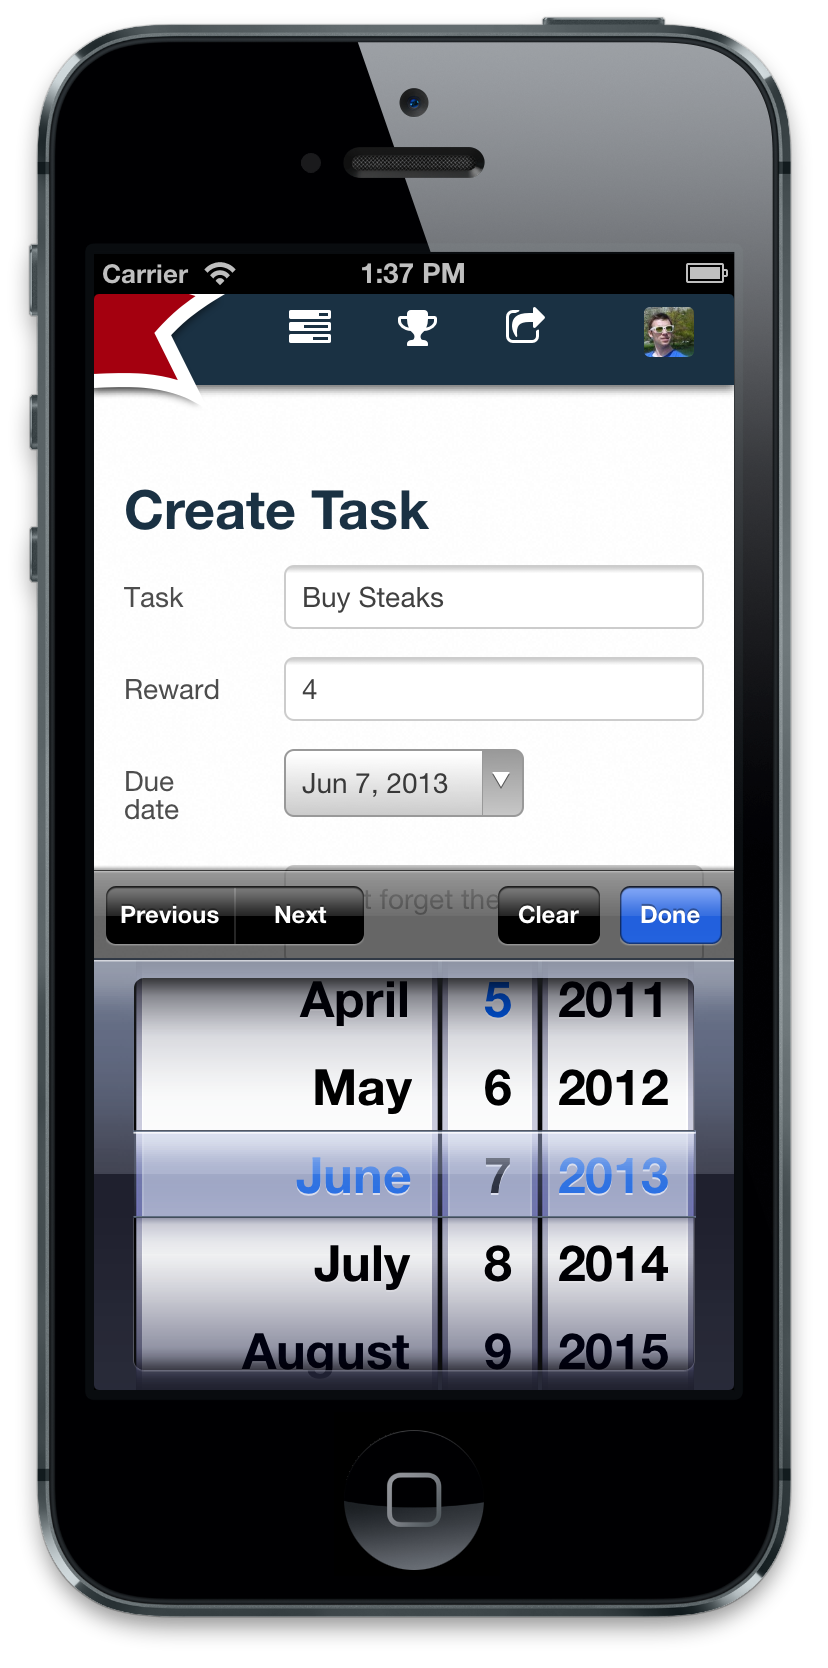
\includegraphics[width=6cm]{content/principle-demonstration/images/iossafari-datepicker.png}
	\caption{Datumsauswahl für ein Textfeld vom Typ \emph{date} in \emph{Safari für iPhone}}
	\label{fig:iossafari-datepicker}
\end{figure}


\subsubsection*{CSS}

Der erstellte CSS Quellcode macht von den neusten CSS 3 Features ausführlichen Gebrauch. So wird für die Darstellung von visuellen Effekten oft auf \emph{box-shadow} oder halbtransparente Farben zurückgegriffen.

Verschiedene Internetbrowser interpretieren CSS Formatierungsbefehle teilweise immer noch sehr unterschiedlich. Um diesem Problem beizukommen wurde die SASS Funktionsbibliothek \emph{Bourbon} \cite{bourbon} eingesetzt. Verschiedene Mixins ermöglichen mit der Verwendung des SASS Präprozessors \cite{SASS} das Generieren von crossbrowser-kompatiblem CSS Quelltext.

\begin{lstlisting}[language=JavaScript, firstnumber=4, caption={Einbindung des \emph{@border-radius} Mixins von \emph{Bourbon} \cite{RoomiesSassBorderRadiusMixin}}, label={lst:roomiesSassBorderRadiusMixin}]
.button {
	@include button($button-color-bg);
	@include border-radius(8px);
	margin-top: 1px;
\end{lstlisting}

Im Bereich \emph{Responsive Design} wurde keine Lösung von Grund auf selbst entwickelt. Unter Zuhilfenahme der \emph{Foundation} SASS Bibliothek \cite{Foundation} wurde auf einfache Art und Weise ein flexibles User Interface Layout entworfen, welches dynamisch auf die verschiedenen Bildschirmgrössen der Endgeräte reagieren kann.

\begin{figure}[H]
	\centering
	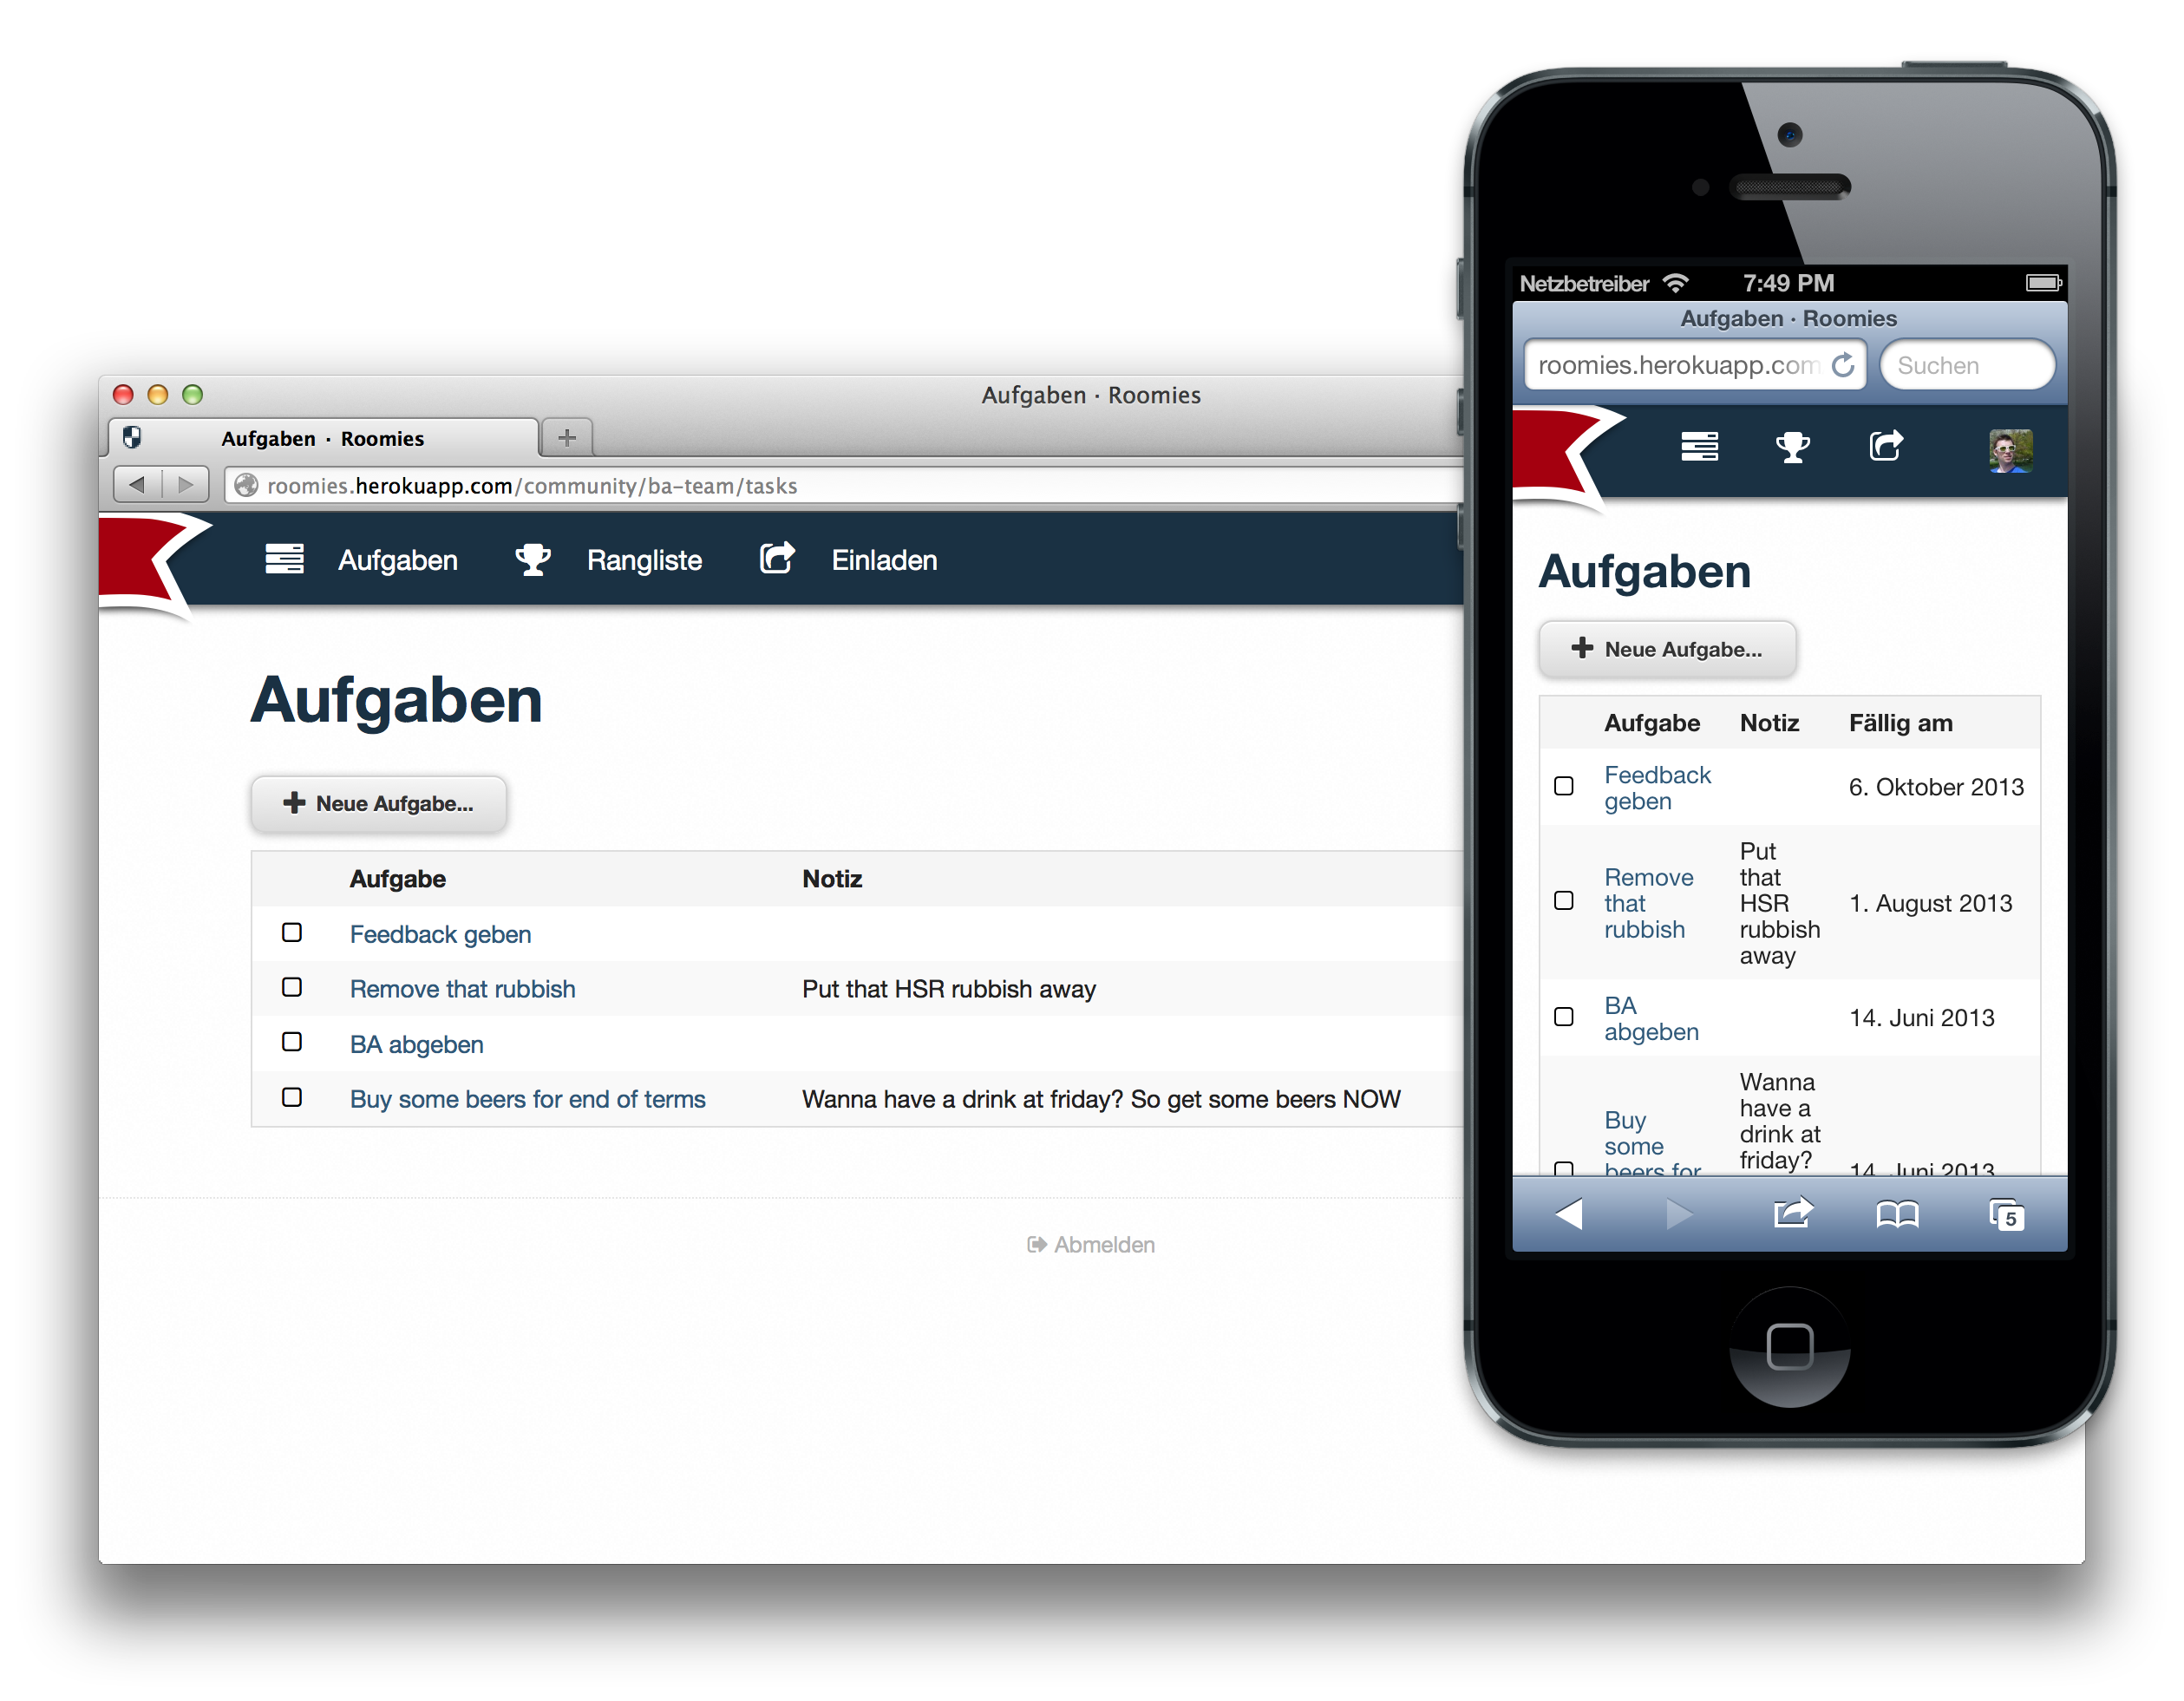
\includegraphics[width=12cm]{content/principle-demonstration/images/responsive-screenshots.png}
	\caption{Media Queries ermöglichen dynamische Anpassung des Layouts entsprechend der verfügbaren Bildschirmgrösse}
	\label{fig:responsive-screenshots}
\end{figure}


\subsubsection*{Navigation mittels Browserfunktionen}

Wie geplant konnte ein einheitliches Navigationsverhalten implementiert werden. Der Benutzer kann sowohl Browsersteuerelemente als auch applikationsinterne Links zur Navigation verwenden, ohne ein unerwartetes Verhalten zu provozieren.

Ausführlichere Informationen zu dieser Thematik sind in Abschnitt \ref{sec:principle-rp10-browser-controls} ``\nameref{sec:principle-rp10-browser-controls}'' sowie \ref{sec:principle-rp18-history-api} ``\nameref{sec:principle-rp18-history-api}'' enthalten.


\subsubsection*{iOS Webapp Kompatibilität}

Zusätzlich zu den geplanten Features wurde die von Apple definierte Spezifikation für \emph{Web Applications} \cite{SafariWebApp} in \emph{Roomies} integriert. Entsprechende Metatags im \emph{<head>}-Bereich des HTML Markups ermöglichen eine bessere Integration der Applikation in die iOS Umgebung. Dazu gehört u.A. ein eigenes Bookmark-Symbol für den iOS Homescreen (siehe Abbildung \ref{fig:webapp-homescreen-icon}) als auch angepasste Ladebildschirme während dem \emph{Aufstarten} der Applikation.

\begin{figure}[H]
	\centering
	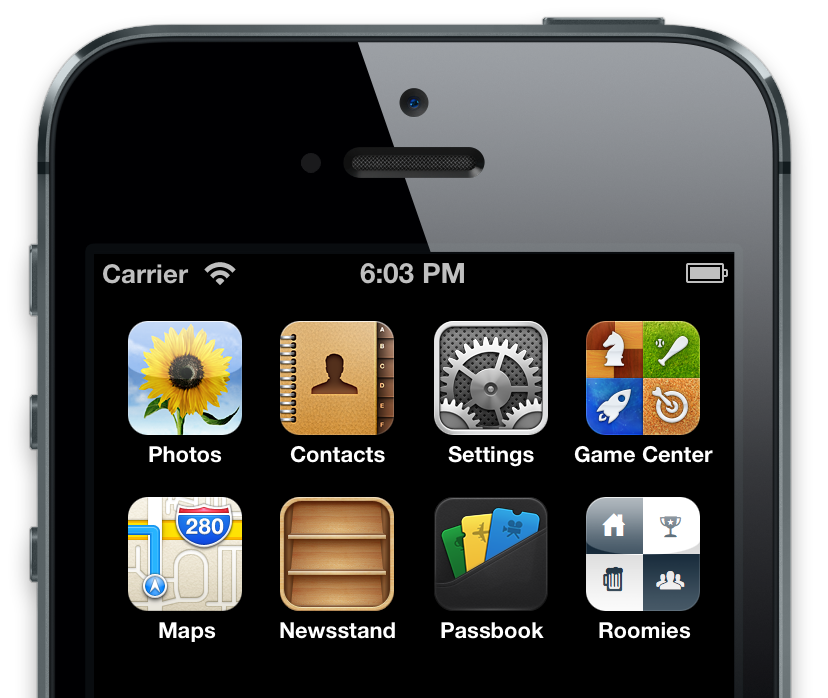
\includegraphics[width=6cm]{content/principle-demonstration/images/ios-webapp-homescreenicon.png}
	\caption{\emph{Roomies} als Webapp auf dem iPhone Homescreen}
	\label{fig:webapp-homescreen-icon}
\end{figure}


\subsection*{Diskussion}

Mächtigere Browser ermöglichen die Ausführung immer ausgefeilterer Internetapplikationen. Umfangreiche Browser API's ersparen die Implementierung eigener Überprüfungsmechanismen für Benutzereingaben oder erleichtern die Gestaltung ansprechender User Interfaces.

In Zukunft wird es zudem vermehrt Möglichkeiten geben, wie vermeintlich schwerfällige Webapplikationen in die Betriebssystemumgebung von Smartphones integriert werden können. Diesbezüglich darf man sehr auf Firefox OS gespannt sein, welches den Ansatz von Apples Webapps auf die Spitze treiben wird \cite{FirefoxOSWebApp}.

Leider scheitern die neuen Standards, welche de facto offiziell noch keine sind, momentan oft an den herstellerspezifischen Implementierungen. So erscheint auf dem iPhone ein benutzerfreundlicher Helfer für die Auswahl eines Datums, in \emph{Mozilla Firefox} \cite{CanIUseDateInput} wird das Datumseingabefeld weiterhin als einfaches Textfeld angezeigt. Für eine Webapplikation hat dies zur Folge, dass im Client weiterhin Logik für die Überprüfung von Benutzereingaben implementiert werden muss. Unter dem Aspekt von Sicherheitsmassnahmen mag dies grundsätzlich logisch erscheinen, bedeutet aber trotzdem erhöhten Aufwand im Entwicklungsprozess.

Viele der neuen Browserfeatures können bereits heute angewendet werden. Durch die mangelnde Standardisierung unter den verschiedenen Browserherstellern ergibt sich für das Projektteam jedoch ein eher durchzogener Eindruck der Situation auf diesem Gebiet.

Aus diesem Grund ermutigt das Projektteam neuste Funktionalitäten zu verwenden, ermahnt jedoch, immer eine Fallbacklösung bereitzuhalten, sollte ein Feature auf einem Browser nicht verfügbar sein.
